

\begin{frame}{Definition}
\Huge
The process of computing and classifying opinions from an unstructured text

\end{frame}
\begin{frame}{Other Names}
\begin{itemize}
\item Opinion mining
\item Evaluation Analysis
\item Appraisal Assessment
\item Attitude mining
\item Emotion extraction
\item Subjectivity analysis
\item Aspect extraction
\item Affect extraction
\item Review mining
\item $\cdots$
\end{itemize}
\end{frame}
% Slide 1: Core Concepts
\begin{frame}{Core Concepts}
    \begin{itemize}
        \item Sentiment reflects emotional tone of text
        \item Polarity: positive, negative, or neutral
        \item Emotion detection for joy, anger, sadness
        \item Aspect-based sentiment: specific components focus
        \item Analyzed at document, sentence, phrase level
    \end{itemize}
\end{frame}

\begin{frame}{Formal definition}
\begin{itemize}
        \item An opinion consists of a \clrtxt{yellow}{target} and \clrtxt{yellow}{sentiment}.
        \item \clrtxt{yellow}{Target (g):} Entity or aspect opinion is about.
        \item \clrtxt{yellow}{Sentiment (s):} Positive, negative, neutral, or numeric score.
        \item Example: 1-5 stars or sentiment polarity.
        \item \clrtxt{yellow}{Polarity types:} Positive, negative, or neutral sentiment.
        \item Targets can include entire entities or specific aspects.
        \item Example: Target in "Canon G12" is \clrtxt{yellow}{camera}.
        \item Example: Target in "Picture quality" is \clrtxt{yellow}{image aspect}.
    \end{itemize}
\end{frame}
\begin{frame}{Target Domain Examples}
\clrtxt{cyan}{Sentiments on the attributes of products}
\begin{itemize}
\item Example: Mobile phone case - design, fitment, price, durability, protection,  shell type (poly carbonate, plastic), color, weight, etc.
\end{itemize}

\clrtxt{cyan}{Services}
\begin{itemize}
\item Banks, restaurants, sports centers, fitness centers, repair shops, etc.
\end{itemize}

\clrtxt{cyan}{Individuals}
\begin{itemize}
\item Example: Fitness instructors/trainers, teachers,
\end{itemize}

\clrtxt{cyan}{Public Issues}
\begin{itemize}
\item Political, non-political, governance, etc.
\end{itemize}
\clrtxt{cyan}{Social media}
\begin{itemize}
\item Monitoring social media for issues, products, trends, etc
\end{itemize}
\clrtxt{cyan}{Events}
\begin{itemize}
\item Music events, workshops, Topics
\end{itemize}


$\Huge \cdots$

\end{frame}


\begin{frame}{Samples}
\begin{center}
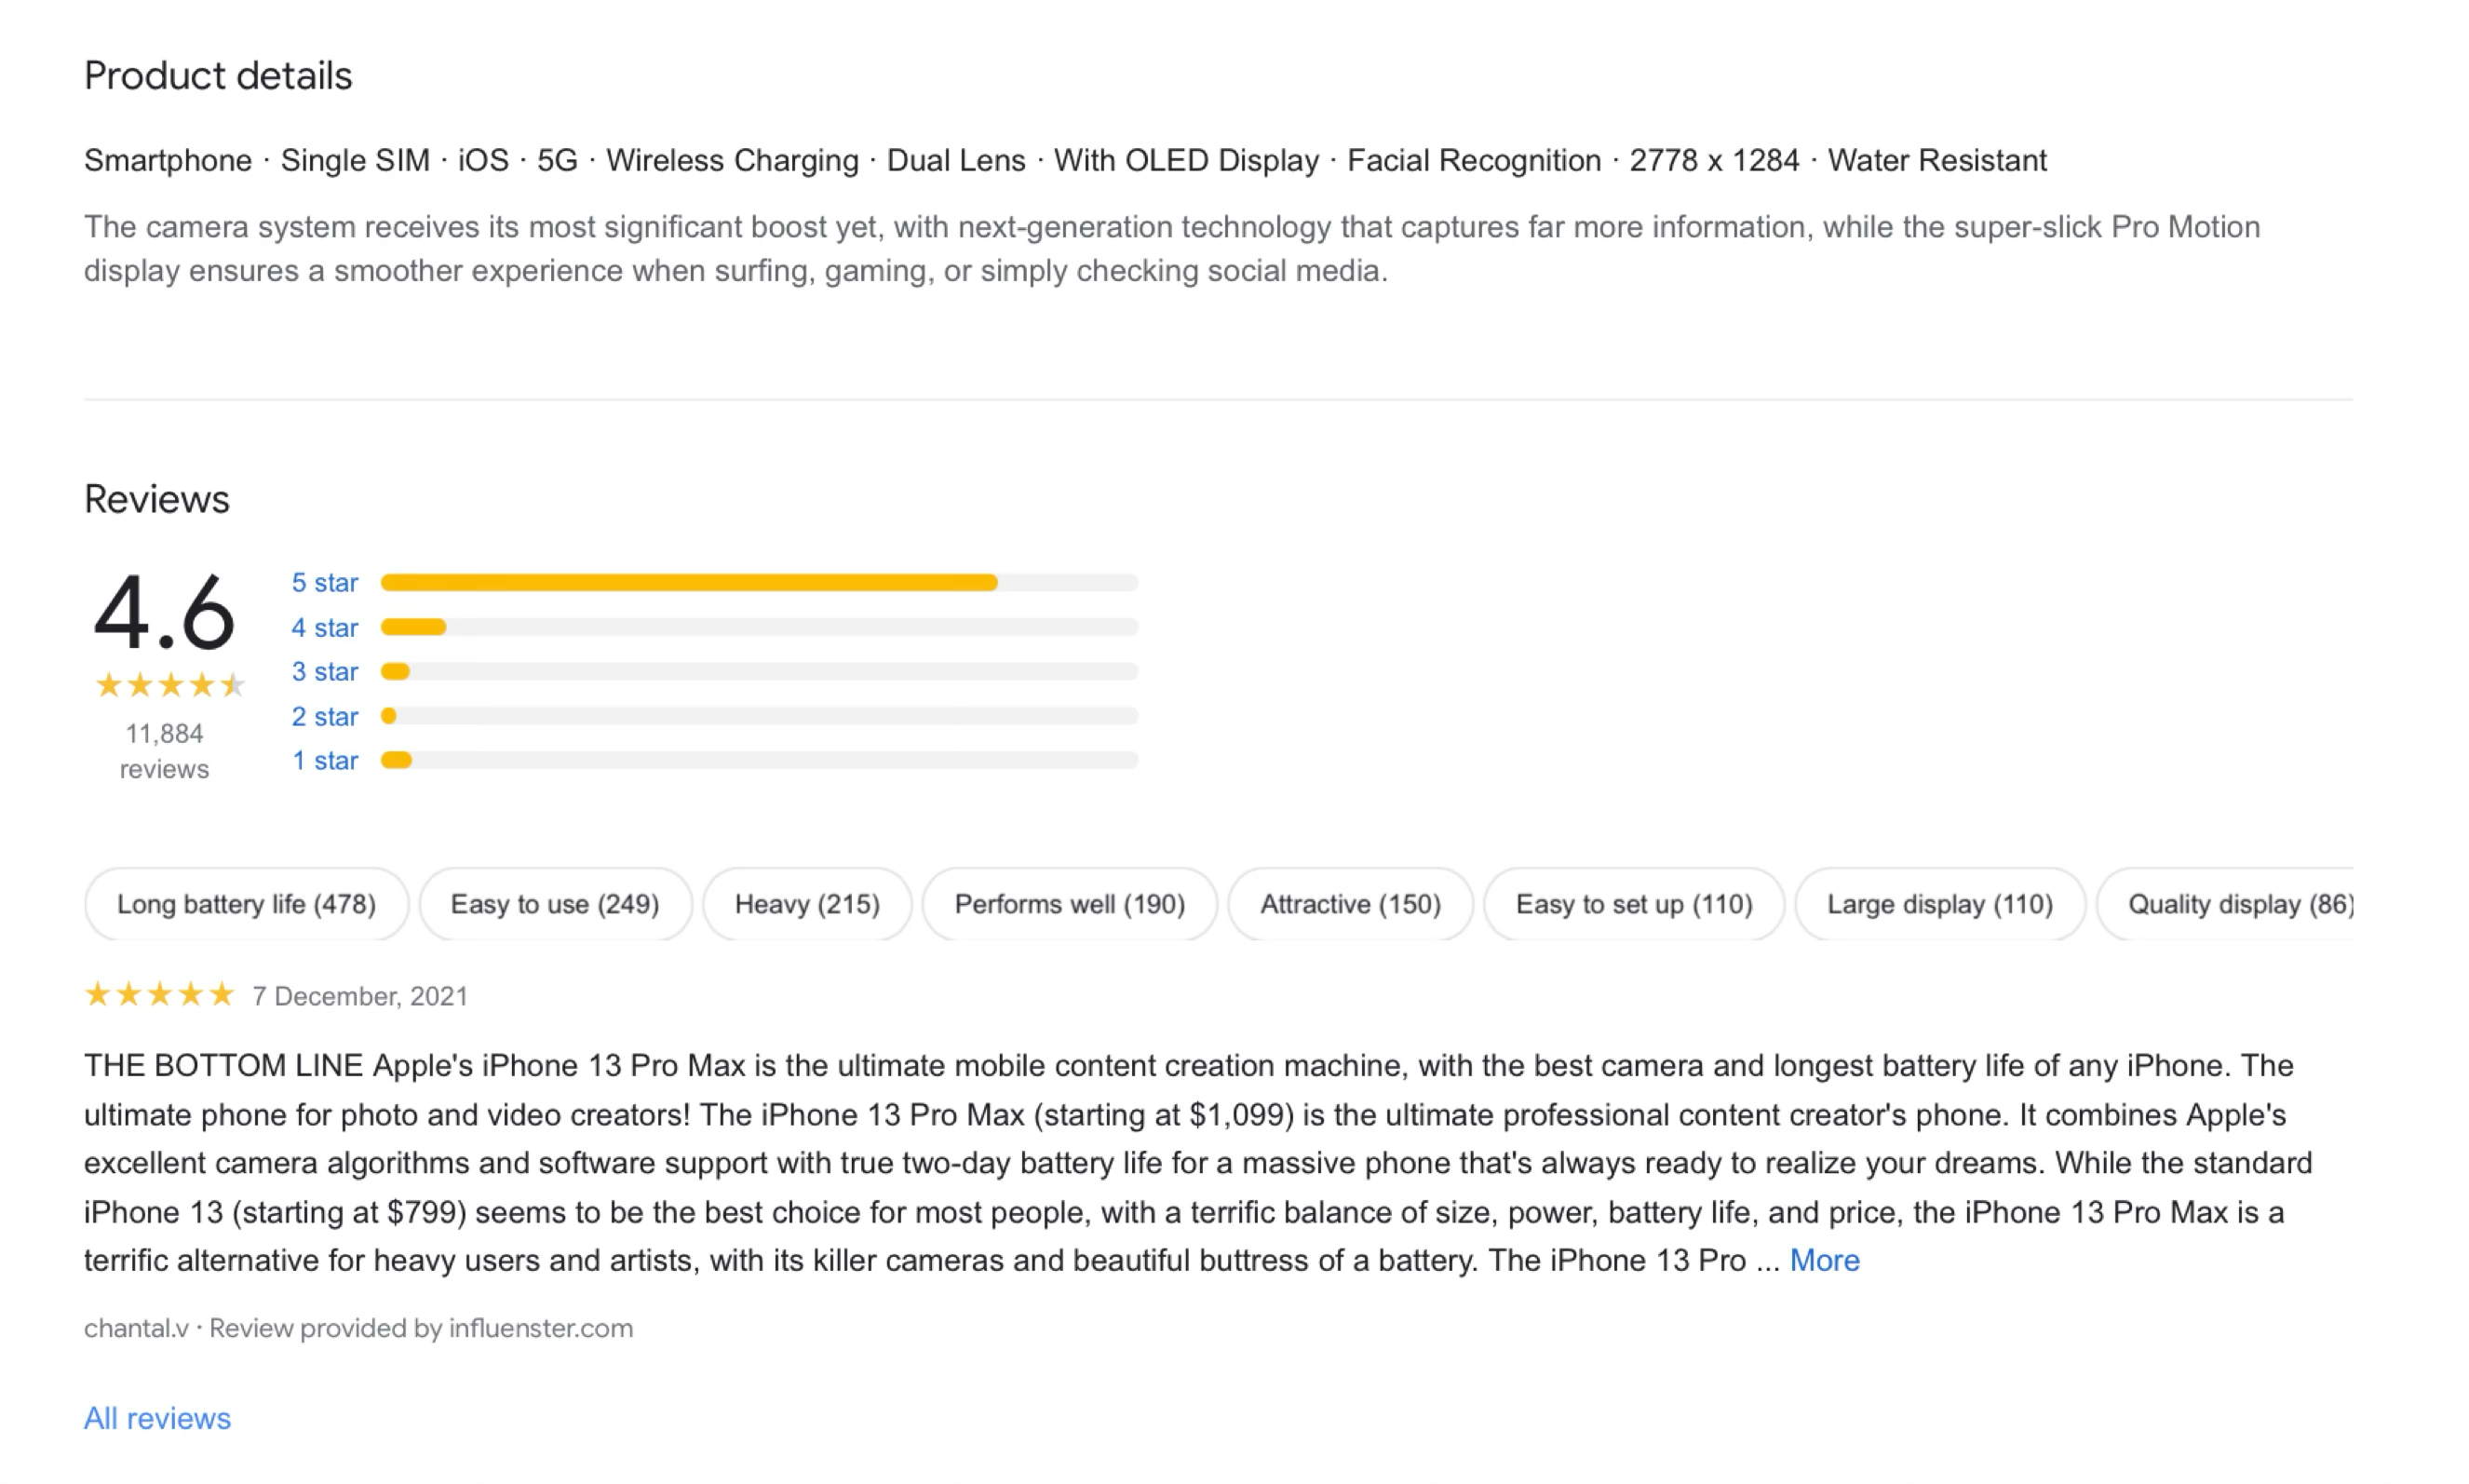
\includegraphics[width=0.85\linewidth]{Images/SAExample1}
\end{center}

\end{frame}

\begin{frame}{Sentiments on attributes}
\begin{center}
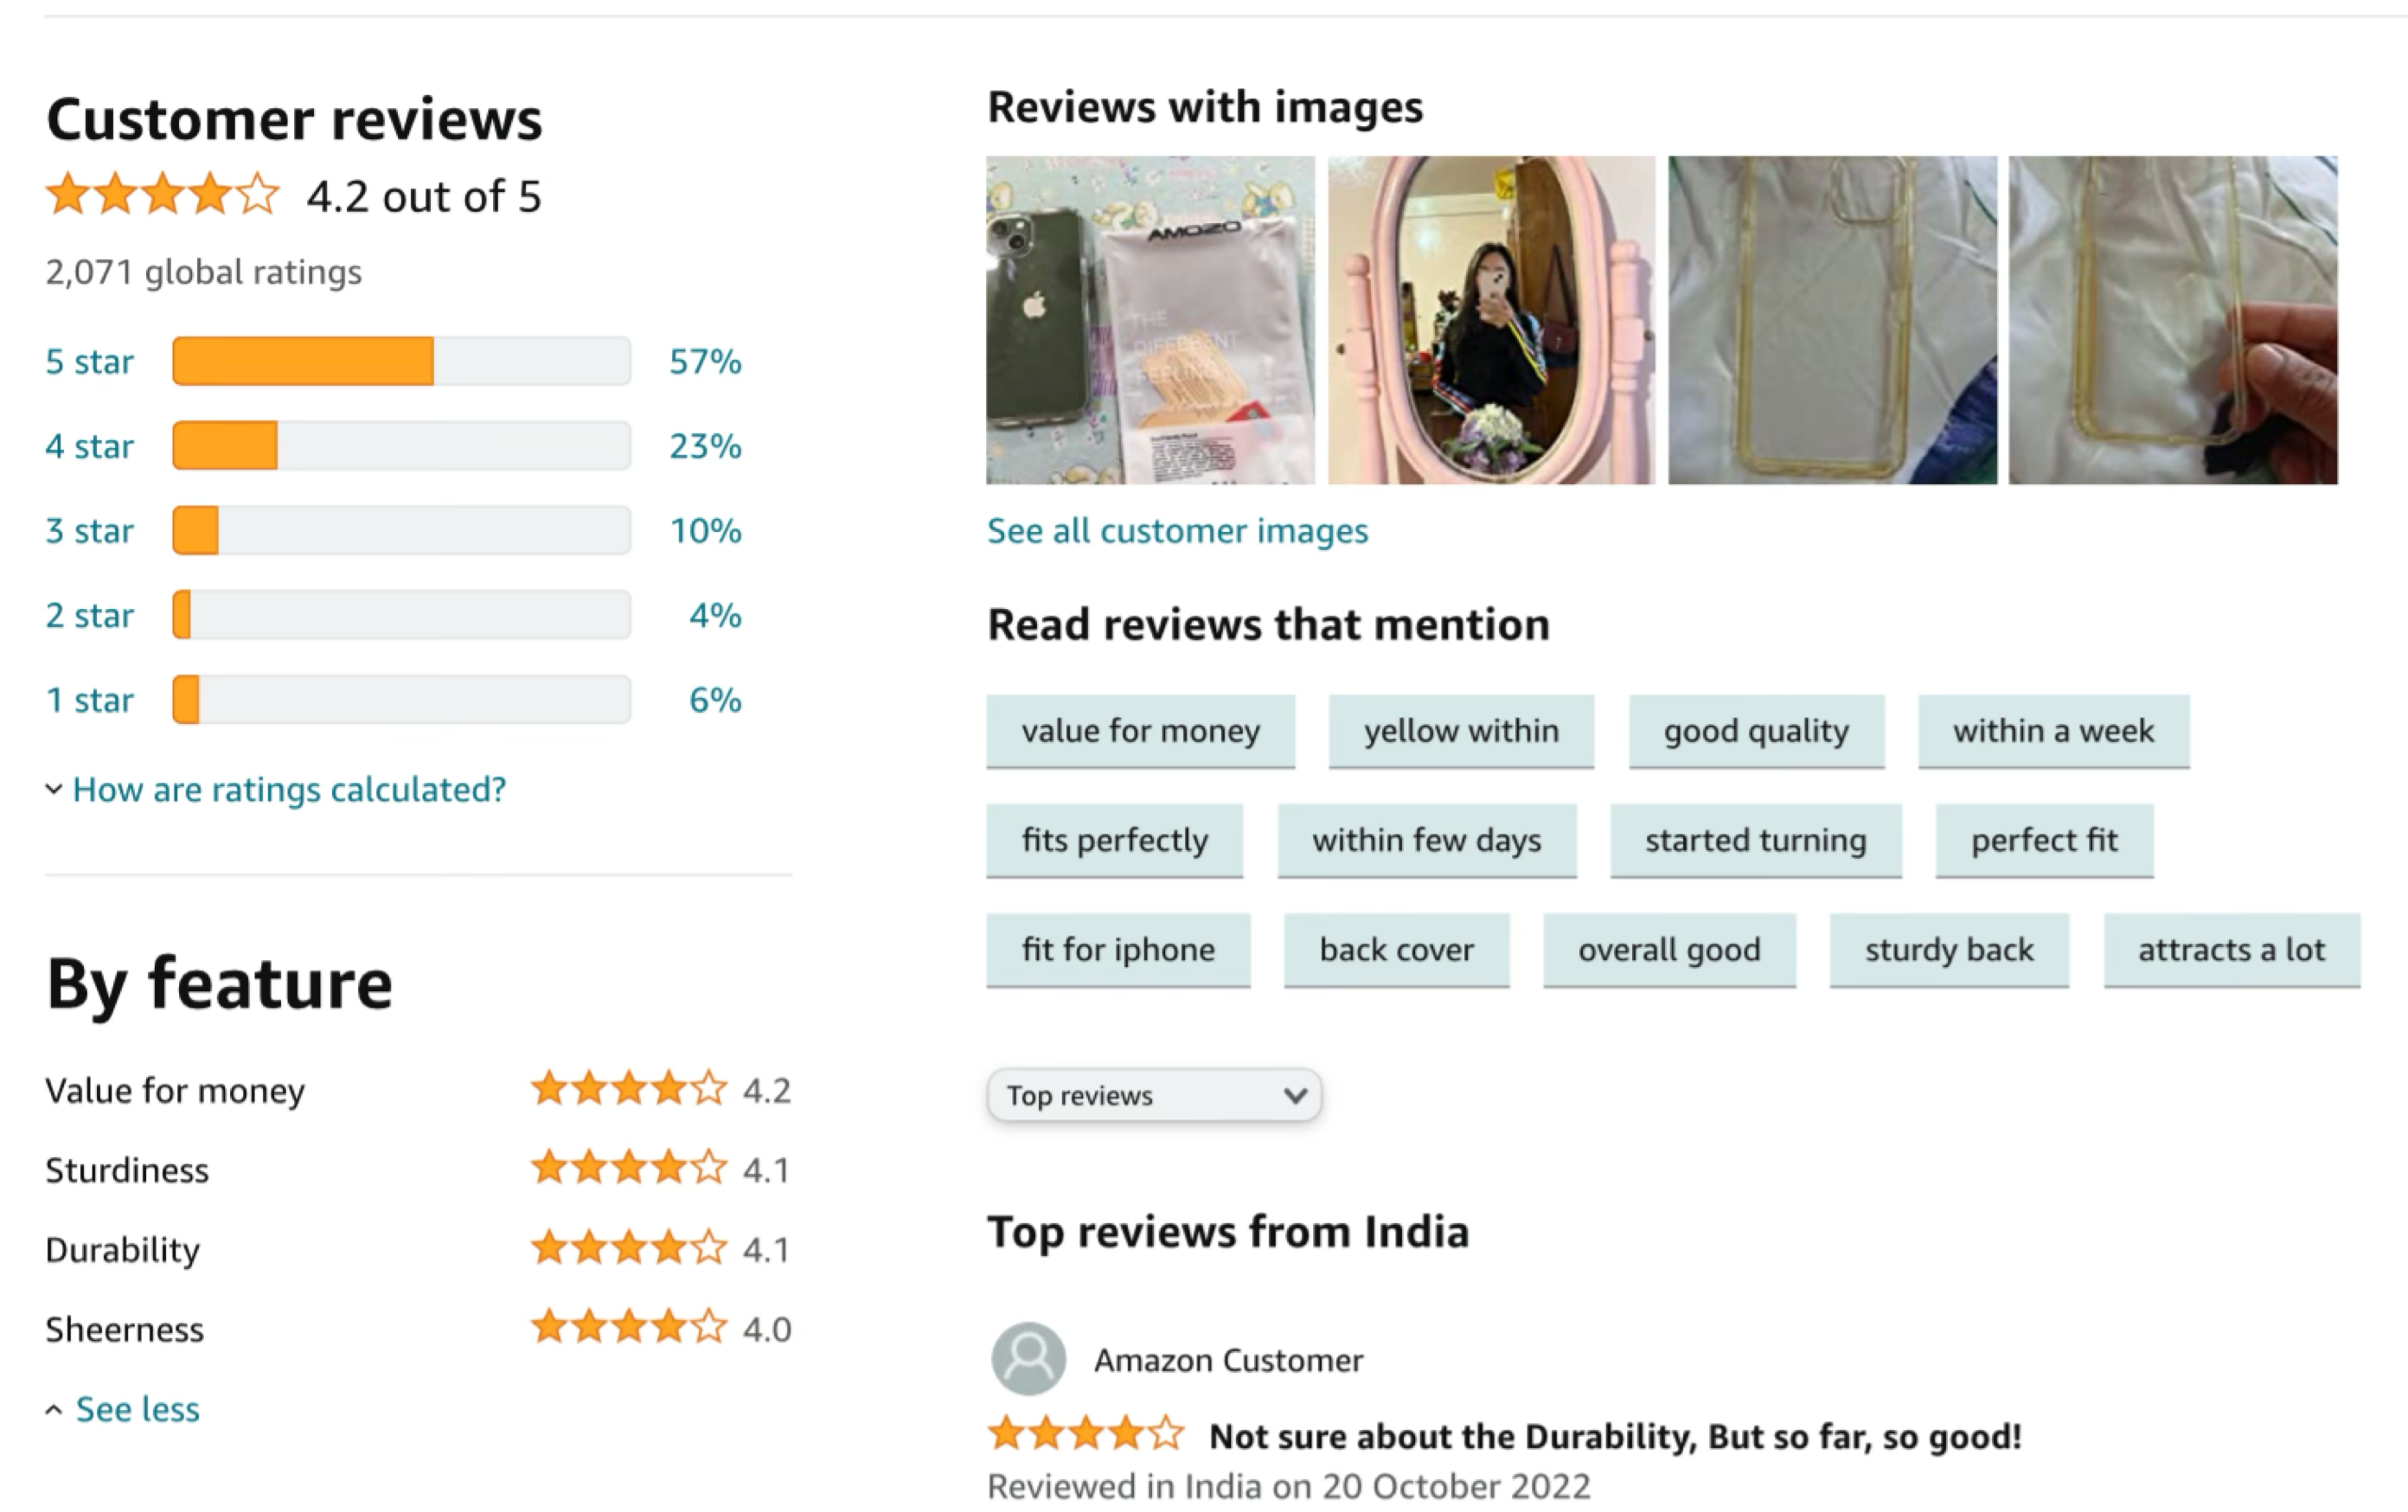
\includegraphics[width=0.85\linewidth]{Images/SAExample2}
\end{center}

\end{frame}

\begin{frame}{Sentiments on Attributes 2/2}
\begin{center}
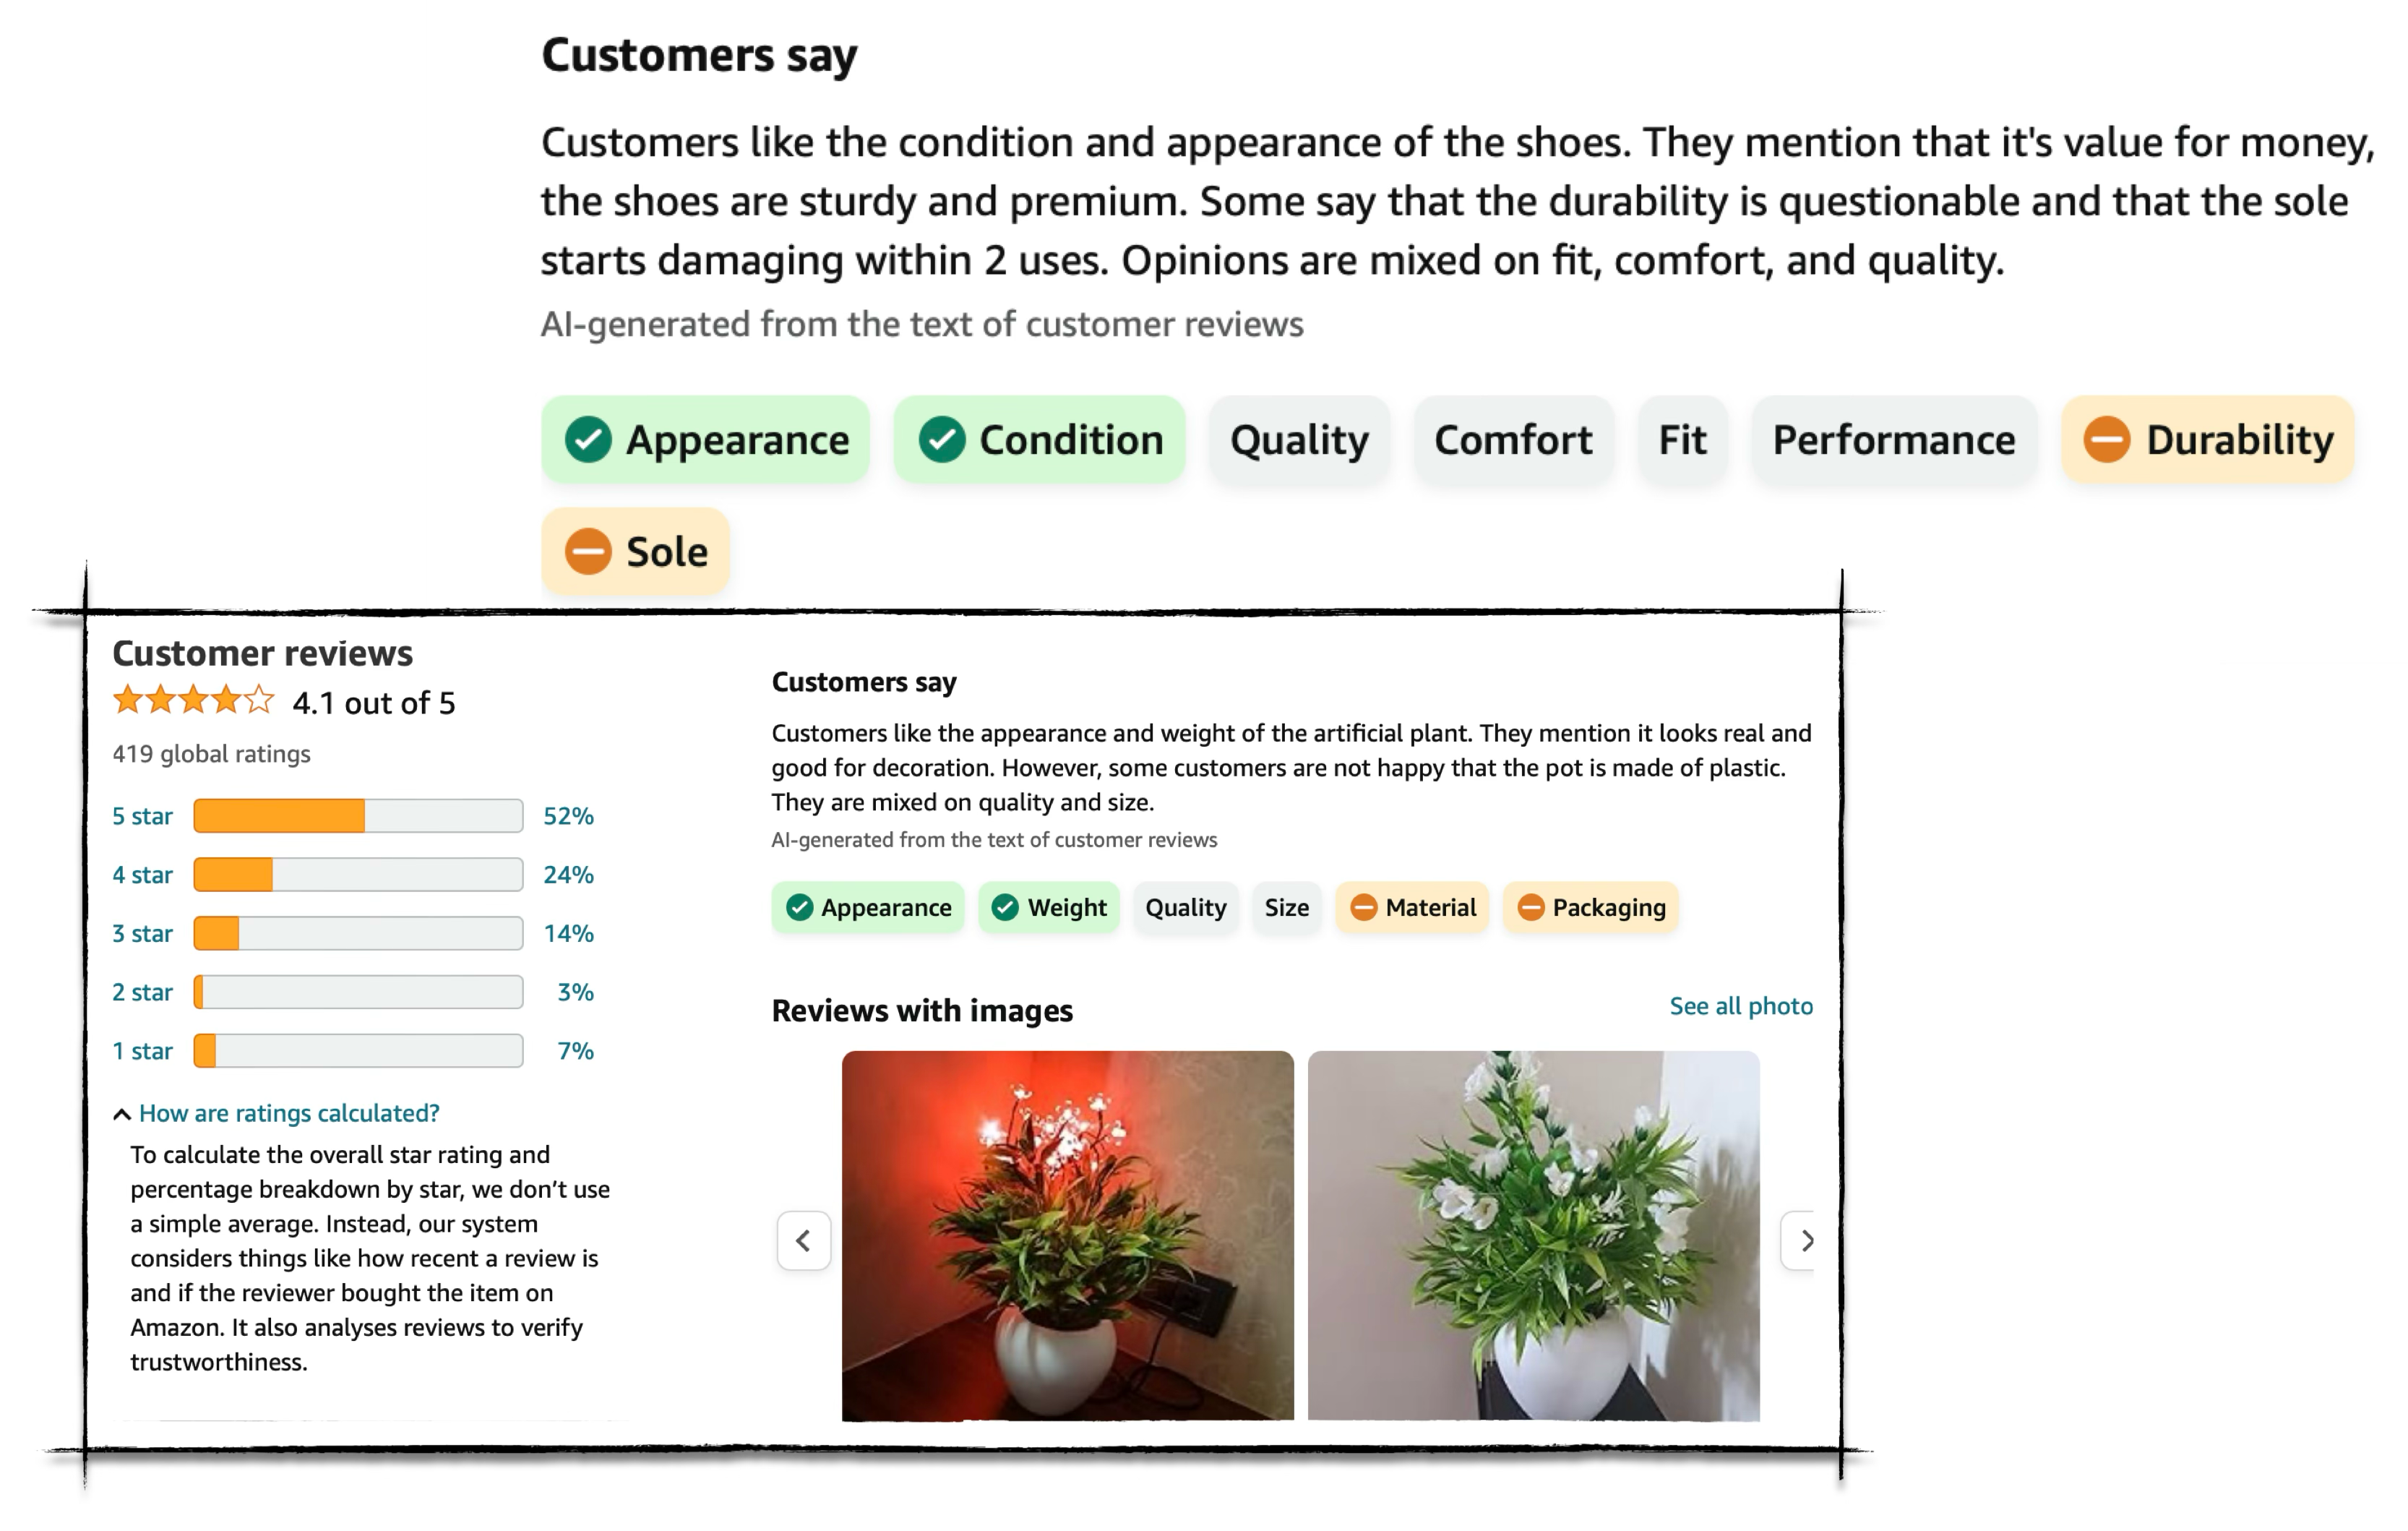
\includegraphics[width=0.85\linewidth]{Images/SAExample3}
\end{center}

\end{frame}


\begin{frame}{Sample Sentences}
\begin{itemize}
\item When you don’t want to spend a whole lot of cash but want a great deal….
\item This is the shop to buy from
\item It is a very cute case
\item Cannot argue with the price or appearance
\item The jewels do fall off
\item It is a beautiful phone case but it is also hard to remove
\item Arrived broken and very flimsy
\item Fits perfectly but needs a little attention at the installation
\item The design and color combination makes the case simple yet elegant, and not too bold and flashy
Don’t believe that these screen protectors have glue in them
\end{itemize}
\end{frame}


\begin{frame}{Sentiment Analysis as a Classification Problem}
    \begin{itemize}
        \item Sentiment analysis can be treated as a    \clrtxt{yellow}{classification task}.
        \item Assigns input text into predefined sentiment categories.
        \item [] \clrtxt{yellow}{Examples of sentiment categories}
        \begin{itemize}
            \item Positive
            \item Negative
            \item Neutral
        \end{itemize}
        \item Classification output can also be represented on a \clrtxt{yellow}{\underline{numerical scale}}.
    \end{itemize}
    \begin{figure}
    \centering
    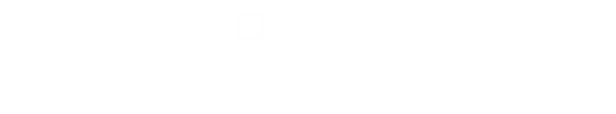
\includegraphics[width=0.7\linewidth]{Images/SAScale}
    \caption{The labeling interface\cite{socher-etal-2013-recursive}}
    \label{fig:sascale}
    \end{figure}


\end{frame}

\begin{frame}{Why Use a Scale?}
    \begin{itemize}
        \item Provides finer granularity than simple positive, negative, or neutral labels.
        \item Enables better differentiation between sentiments of similar types.
        \item Allows for more nuanced analysis, e.g., distinguishing between slightly positive (+5) and highly positive (+20).
        \item Facilitates advanced tasks like regression-based sentiment prediction.
    \end{itemize}
\end{frame}

\begin{frame}{Approaches to Sentiment Analysis}
    \begin{itemize}
        \item Rule-based: lexicons and manual rules
        \item Machine learning: Naive Bayes, SVM, others
        \item Deep learning: CNNs, RNNs, Transformers
        \item Trade-offs: simplicity vs. computational complexity
    \end{itemize}
\end{frame}


\begin{frame}{Challenges}
    \begin{multicols}{2}
    \begin{itemize}
        \item Context impacts interpretation of sentiment
        \item Sarcasm and irony are difficult to detect
        \item Sentiment varies across different domains
        \item Handling ambiguous and mixed sentiments is tricky
        \item Multilingual and multimodal sentiment needs innovation
    \end{itemize}
    \vfill\null
    \columnbreak
    \begin{center}
    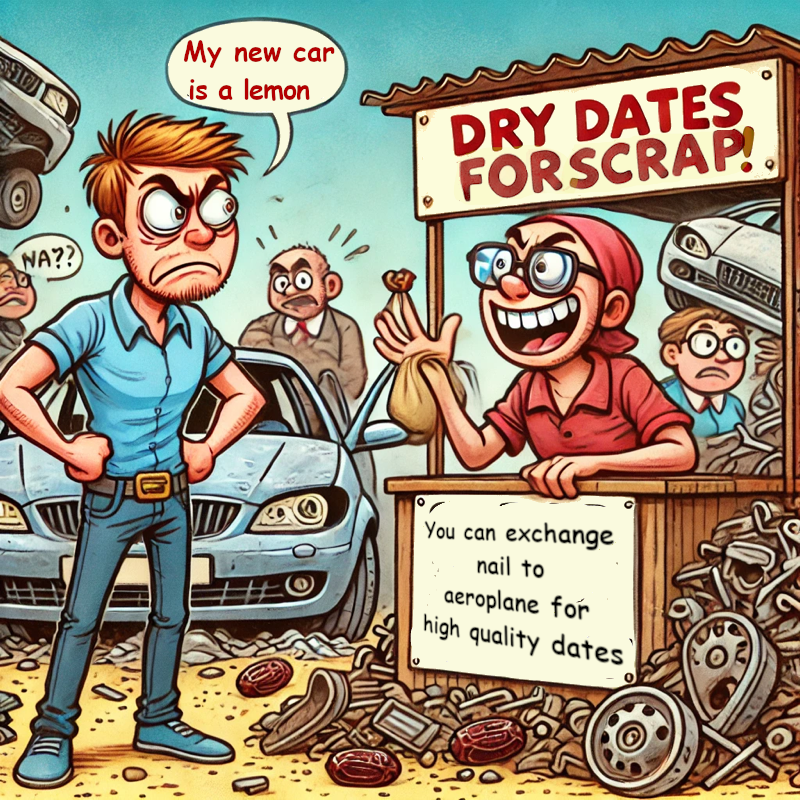
\includegraphics[width=0.7\linewidth]{Images/SAJoke}
    \end{center}

    \end{multicols}
\end{frame}

% Slide 4: Applications
\begin{frame}{Applications}
    \begin{itemize}
        \item Analyze customer reviews for feedback insights
        \item Monitor political opinions and public reactions
        \item Assess sentiment in healthcare and treatments
        \item Predict audience reactions to entertainment content
        \item Monitor brand sentiment on social media
    \end{itemize}
\end{frame}

% Slide 5: Tools and Libraries
\begin{frame}{Tools and Libraries}
    \begin{itemize}
        \item TextBlob: easy sentiment classification library
        \item VADER: social media sentiment lexicon-based tool
        \item NLTK: preprocessing and sentiment classification
        \item Commercial APIs: IBM Watson, AWS Comprehend
    \end{itemize}
\end{frame}

\begin{frame}{Taxonomy}
\begin{figure}
\centering
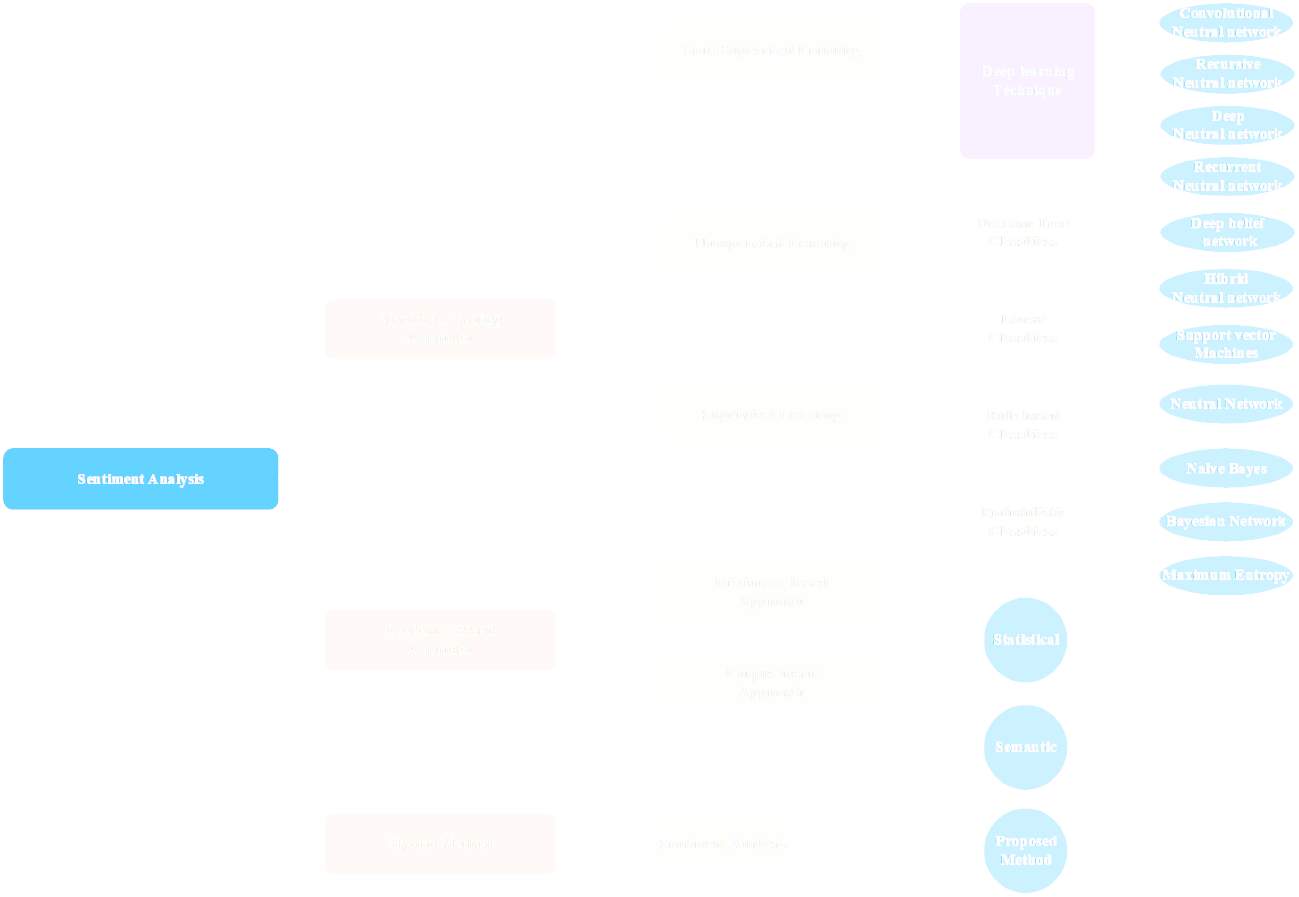
\includegraphics[width=0.7\linewidth]{Images/SATaxonomy}
\caption[SATaxonomy]{Taxonomy of sentiment analysis techniques\cite{Dang_2020}.}
\label{fig:sataxonomy}
\end{figure}
\end{frame}

\begin{frame}{Traditional Approaches}

\begin{itemize}
    \item Lexicon based Approach
    \item {Naive Bayes Classifier}
	\item Support Vector Machines (SVM)
	\item Effective in high-dimensional spaces for binary or multi-class classification
	\item Logistic Regression
	\item Decision Trees and Random Forests
	\item K-Nearest Neighbors (KNN)
\end{itemize}
\end{frame}

\begin{frame}{Future Directions}
    \begin{itemize}
        \item Combining text, voice, and video sentiment
        \item Real-time sentiment analysis for live events
        \item Summarizing sentiment across vast datasets
        \item Enhancing model explainability and transparency
    \end{itemize}
\end{frame}
